\documentclass[tikz,border=2mm]{standalone}
\usetikzlibrary{arrows.meta,calc,shapes.geometric}

\begin{document}

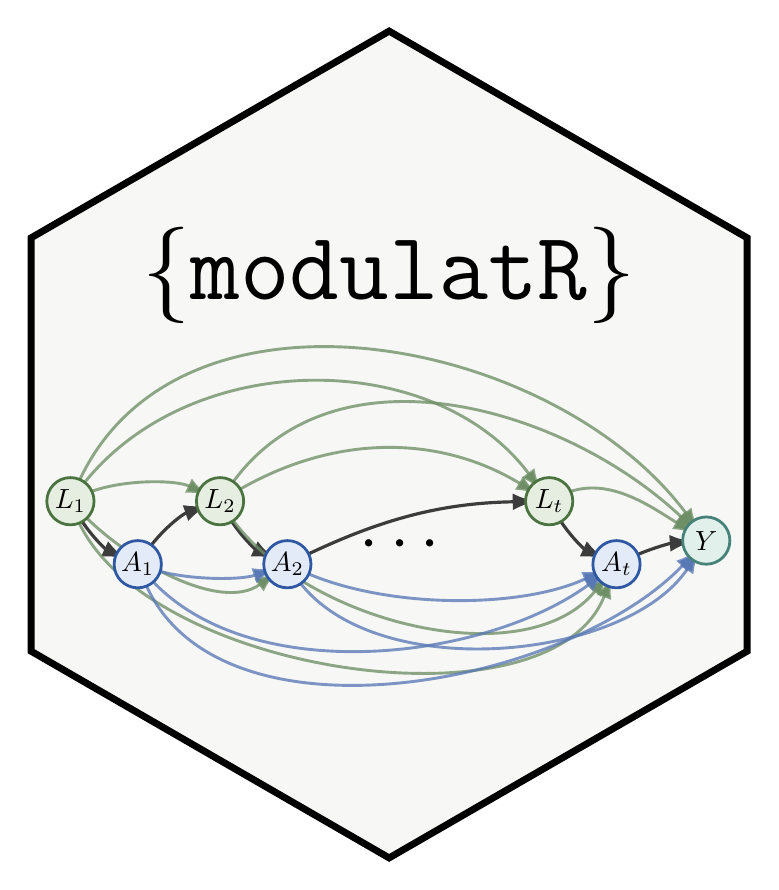
\begin{tikzpicture}[>=Latex]

% Colors
\definecolor{hexbg}{RGB}{247,247,245}
\definecolor{Ldraw}{RGB}{74,115,64}
\definecolor{Lfill}{RGB}{229,238,225}
\definecolor{Adraw}{RGB}{47,88,163}
\definecolor{Afill}{RGB}{227,234,248}
\definecolor{Ydraw}{RGB}{70,130,120}
\definecolor{Yfill}{RGB}{226,240,236}
\definecolor{mainarrow}{RGB}{60,60,60}

% Styles
\tikzset{
  Lnode/.style={
    circle,
    draw=Ldraw,
    fill=Lfill,
    line width=1pt,
    minimum size=6mm,
    inner sep=0pt,
    font=\normalsize
  },
  Anode/.style={
    circle,
    draw=Adraw,
    fill=Afill,
    line width=1pt,
    minimum size=6mm,
    inner sep=0pt,
    font=\normalsize
  },
  Ynode/.style={
    circle,
    draw=Ydraw,
    fill=Yfill,
    line width=1pt,
    minimum size=6mm,
    inner sep=0pt,
    font=\normalsize
  },
  direct/.style={
    ->,
    line width=1.15pt,
    draw=mainarrow,
    shorten >=5pt,
    shorten <=5pt
  },
  Larrow/.style={
    ->,
    line width=1.05pt,
    draw=Ldraw!80,
    draw opacity=0.78,
    shorten >=5pt,
    shorten <=5pt
  },
  Aarrow/.style={
    ->,
    line width=1.05pt,
    draw=Adraw!80,
    draw opacity=0.78,
    shorten >=5pt,
    shorten <=5pt
  }
}

% Hexagon
\node[
  regular polygon,
  regular polygon sides=6,
  shape border rotate=30,
  draw=black,
  fill=hexbg,
  line width=2.5pt,
  minimum width=10.5cm,
  minimum height=9.2cm,
  inner sep=0pt
] (hex) at (0,0) {};

% Title
\node[
  scale=1.4,
  font=\ttfamily\bfseries\fontsize{26}{28}\selectfont
] at ($(hex.center)+(0,2.15)$) {\{modulatR\}};

% Graph
\begin{scope}[shift={($(hex.center)+(-.2,-1.4)$)}]
\begin{scope}[xscale=0.95]

  % Coordinates first, so arrows can be drawn behind nodes
  \coordinate (L1c) at (-4.05,  0.68);
  \coordinate (A1c) at (-3.15, -0.12);

  \coordinate (L2c) at (-2.05,  0.68);
  \coordinate (A2c) at (-1.15, -0.12);

  \coordinate (dotsc) at (0.35, 0.12);

  \coordinate (Ltc) at (2.35,  0.68);
  \coordinate (Atc) at (3.25, -0.12);

  \coordinate (Yc)  at (4.45,  0.18);

  % ----------------------------
  % Arrows first, nodes later
  % ----------------------------

  % Direct/local arrows
  \draw[direct] (L1c) to[bend right=18] (A1c);
  \draw[direct] (A1c) to[bend left=18]  (L2c);
  \draw[direct] (L2c) to[bend right=18] (A2c);
  \draw[direct] (A2c) to[bend left=12]  (Ltc);
  \draw[direct] (Ltc) to[bend right=18] (Atc);
  \draw[direct] (Atc) to[bend left=10]  (Yc);

  % Top lane: L-history arrows to future L's
  \draw[Larrow] (L1c) to[out=25,in=155,looseness=0.85] (L2c);
  \draw[Larrow] (L2c) to[out=30,in=150,looseness=1] (Ltc);
  \draw[Larrow] (L1c) to[out=52,in=128,looseness=1] (Ltc);

  % Highest lane: L-history arrows to Y
  \draw[Larrow] (L1c) to[out=66,in=128,looseness=1] (Yc);
  \draw[Larrow] (L2c) to[out=55,in=138,looseness=1] (Yc);
  \draw[Larrow] (Ltc) to[out=25,in=150,looseness=1] (Yc);

  % Lower green lane: L-history arrows into future A's
  \draw[Larrow] (L1c) to[out=-45,in=-145,looseness=0.92] (A2c);
  \draw[Larrow] (L2c) to[out=-55,in=-130,looseness=0.90] (Atc);
  \draw[Larrow] (L1c) to[out=-68,in=-112,looseness=0.82] (Atc);

  % Lower blue lane: A-history arrows to future A's
  \draw[Aarrow] (A1c) to[out=-18,in=-162,looseness=0.85] (A2c);
  \draw[Aarrow] (A2c) to[out=-24,in=-156,looseness=0.82] (Atc);
  \draw[Aarrow] (A1c) to[out=-48,in=-145,looseness=0.86] (Atc);

  % Lowest blue lane: A-history arrows to Y
  \draw[Aarrow] (A1c) to[out=-68,in=-135,looseness=0.88] (Yc);
  \draw[Aarrow] (A2c) to[out=-55,in=-125,looseness=0.86] (Yc);

  % Nodes drawn after arrows, so fills hide crossings near node centers
  \node[Lnode] (L1) at (L1c) {$L_1$};
  \node[Anode] (A1) at (A1c) {$A_1$};

  \node[Lnode] (L2) at (L2c) {$L_2$};
  \node[Anode] (A2) at (A2c) {$A_2$};

  \node at (dotsc) {\fontsize{24}{24}\selectfont $\cdots$};

  \node[Lnode] (Lt) at (Ltc) {$L_t$};
  \node[Anode] (At) at (Atc) {$A_t$};

  \node[Ynode] (Y) at (Yc) {$Y$};

\end{scope} % xscale
\end{scope} % graph shift

\end{tikzpicture}

\end{document}
